%% LyX 2.3.7 created this file.  For more info, see http://www.lyx.org/.
%% Do not edit unless you really know what you are doing.
\documentclass[english]{article}
\usepackage[T1]{fontenc}
\usepackage[latin9]{inputenc}
\usepackage{babel}
\usepackage{float}
\usepackage{amsmath}
\usepackage{amssymb}
\usepackage{graphicx}
\usepackage[unicode=true]
 {hyperref}

\makeatletter

%%%%%%%%%%%%%%%%%%%%%%%%%%%%%% LyX specific LaTeX commands.
\newcommand{\noun}[1]{\textsc{#1}}
%% A simple dot to overcome graphicx limitations
\newcommand{\lyxdot}{.}


\makeatother

\begin{document}
\title{\textbf{Study of Josephson Junction }\\
\textbf{- }\\
\textbf{Simulations and analysis }\\
}
\author{\noun{Undergraduate Thesis}}
\author{\medskip{}
\\
Submitted in partial fulfillment of the requirements of\emph{}\\
\emph{BITS F421T Thesis }\\
\emph{By} \\
Ashwin Kumar K\\
ID No. 2017B5A81034G\\
\medskip{}
\\
\emph{Under the guidance of :}\\
\medskip{}
\\
Dr. Kartik Senapati, NISER, Bhubaneswar\\
\emph{\&}\\
Dr. Ramesha C K, BITS Pilani, Goa}

\maketitle
\begin{figure}[H]

\begin{centering}
\includegraphics[width=5cm]{bits_logo}
\par\end{centering}
\end{figure}

\newpage{}

\section*{Declaration}

I, Ashwin Kumar K, declare that this Undergraduate Thesis titled,
`Study of Josephson Junction - Simulations and analysis' and the work
presented in it are my own. I confirm that:
\begin{itemize}
\item This work was done mainly or wholly  while in candidature for a research
degree at this University. 
\item Where any part of this thesis has previously been submitted for a
degree or any other qualification at this University or any other
institution, this has been clearly stated.
\item Where I have consulted the published work of others, this is always
clearly attributed.
\item Where I have quoted from the work of others, the source is always
given. With the exception of such quotations, this         thesis
is entirely my own work. 
\item Where the thesis is based on work done by         myself jointly with
others, I have made clear exactly what was done by         others
and what I have contributed myself.
\item I have acknowledged all main sources of help.

Signed: \\

Date:
\end{itemize}
\newpage{}

\section*{Acknowledgments}

I wish to thank my project supervisors, Dr. Kartikeswar Senapati and
Dr. Ramesha C K for their immense support and help with the understanding
of this project. I would like to express my deepest appreciation to
Mr. Tapas Ranjan Senapati and Ms. Laxmipriya Nanda for all their help
from mentoring on the fabrication techniques to usage of measurement
systems and all the fruitful discussions. I wish to thank all the
lab members of Superconductivity lab, NISER for all the brainstorming
sessions which helped me greatly. Special thanks to Ms. Soheli Mukherjee
who always supported me with all my endeavors. I would also like to
extend my deepest gratitude to Dr. Dhavala Suri who always showered
me with helpful advice. Lastly, I am thankful to all my friends and
family members for extending their love and support.

\newpage{}

\tableofcontents{}

\section*{\newpage}

\section*{Abbreviations}
\begin{itemize}
\item AC :- Alternating current 
\item RF :- Radio frequency 
\item JJ :- Josephson Junction
\item SQUID :- Superconducting QUantum Interference Device
\item EDX :- Energy Dispersive X-ray spectroscopy 
\item SEM :- Scanning Electron Microscope
\item FIB :- Focused Ion Beam 
\item PPMS :- Physical Properties Measurement System 
\item Fig :- Figure 
\item eV :- Electron Volt 
\item KeV :- Kilo Electron Volt 
\item MeV :- Mega/Million Electron Volt 
\item et al :- And others (Latin) 
\item i.e. :- That is 
\item etc :- Et cetera (Latin for \textquoteright and others of same kind\textquoteright ) 
\item T :- Tesla 
\item SiO2:- Silicon dioxide
\item R-T :- Resistance Versus Temperature 
\item I-V :- Current Versus Voltage 
\item I-H :- Current Versus Magnetic field 
\item V-H :- Voltage Versus Magnetic field 
\item Si :- Silicon 
\item K :- kelvin
\item mm :- millimeter 
\item mbar :- millibar 
\item IPA :- Isopropyl alcohol 
\item RPM :- Revolutions Per Minute 
\item C :- Celsius 
\item Ar :- Argon 
\item e.g. :- Example given 
\item TSP :- Titanium Sublimation Pump 
\item RGA :- Residual Gas Analyzers 
\item Cu :- Copper 
\item BCS :- Bardeen--Cooper--Schrieffer 
\item Nb :- Niobium 
\item DC :- Direct current
\item AC :- Alternating current
\item $\mu$A :- Micro Ampere 
\item $\Omega$:- Ohm 
\item nm :- Nano meter
\end{itemize}
\newpage{}

\part{Introduction}

At the beginning of this thesis, we introduce basic theoretical concepts
that underlay the device we are trying to study, i.e. the Josephson
Junction (JJ). We first study the postulates of superconductivity.
Then we look at the Josephson effect, which describes the physics
of a Superconductor-Insulator-Superconductor sandwich and then look
at a popular model of a realistic Josephson junction, namely the RCSJ
model. Later we will try to understand various aspects of fabrication
and characterisation of such devices.

\section{Superconductivity}

Heike Kamerlingh Onnes discovered the phenomenon of superconductivity
in the Netherlands in 1911. He was the first to observe that the electrical
resistance becomes exactly zero in certain materials and in temperatures
below a specific critical value $T_{c}$ \cite{Tinkham-1}. Soon after
this discovery, several other materials that showed superconducting
behaviour were discovered, with different critical temperatures. Currently
the highest temperature at which superconductivity was observed is
in hydrogen sulphide ($H_{2}S$), which has a $T_{c}$ reported as
203K, but at extremely high pressures \cite{HighTc}. In 1933, Meissner
and Ochsenfeld discovered that within a superconductor, the magnetic
field completely vanishes i.r becomes zero, making the superconductor
a perfect diamagnet. The expulsion of a magnetic field inside a superconductor
is called the Meissner effect. Then the London brothers explained
this effect, who proved that the magnetic field inside a superconductor
has an exponential decay from the surface, with a decay length $\lambda$,
called London penetration depth. They explained that in order to facilitate
this, the superconductor sets up electric currents on its surface,
whose magnetic field opposes and cancels the applied magnetic field
within the superconductor. The phenomenon of superconductivity was
theoretically explained in 1957, almost 46 years after its initial
discovery, by Bardeen, Cooper, and Schrieffer \cite{BCS}. They proposed
the first microscopic theory of superconductivity, which was named
the BCS theory, and received the Nobel Prize in Physics in 1972. They
suggested that the electrons of a superconductor that are close to
the Fermi surface attract indirectly through the crystal lattice,
which is mediated by the exchange of phonons. This attraction overcomes
the Coulomb repulsion between the two electrons and the electrons
form pairs, which we now call as Cooper pairs. Cooper pairs feel no
scattering, and thus lead to the formation of supercurrent. In $T>T_{c}$
though, the thermal vibration energy of the lattice becomes more significant
than the pairing energy of the electrons, so the Cooper pair breaks,
and thus the material becomes normal. It was later discovered that
superconducting materials behave in different ways upon application
of external magnetic fields. There are two major categories of superconductors
which are type I and type II. A type I has only one critical field
(keeping other parameters like current density and temperature constant)
above which all superconductor properties are lost and while in superconducting
state all magnetic field lines or magnetic flux are completely pushed
out from the bulk of the material. In the case of a type II superconductor,
there exists two separate critical field values between which a single
flux quanta, $\phi_{0}$, of the magnetic field is allowed to pass
through the superconductor through isolated points and are called
vortices. Currently one of the most used applications of superconductivity
is to produce extremely high magnetic fields ranging into tens of
teslas can trace it\textquoteright s origin back to 1955 when G. B.
Yntema created the first ever superconducting electromagnet using
superconducting Nb wire windings with an iron-core, this setup was
outputting a 0.7 T magnetic field

\section{Josephson Junctions}

Prior to 1962, researchers were familiar with quantum mechanical tunneling
of normal electrons through a weak barrier; however, the probability
of tunneling of a cooper pair was thought to be insignificant given
that the pair as a whole would have to tunnel through the barrier.
In 1962 Brian David Josephson showed that this tunneling probability
is not low as previously thought. He predicted theoretically that
two superconductors that are coupled (are in close proximity) by a
weak link, which link may be made of a normal metal, an insulator,
or a constriction of superconductivity, can still let the super current
flow through them \cite{BDJJ}. This macroscopic phenomenon was given
the name Josephson effect. 
\begin{figure}[H]
\centering{}\includegraphics[width=8cm]{a-The-superconducting-order-parameter-of-a-superconductor-S-penetrating-into-the}\caption{(a) The superconducting order parameter $\Psi$ of a superconductor
(S) penetrating into the normal metal (N) with a length scale of the
superconducting coherence length,$\xi$. (b) Order parameters from
two sides have an overlap in N, producing proximity Josephson coupling.\cite{SCFig}}
\end{figure}

Josephson demonstrated that, for a short junction, the current that
flows through the junction when no voltage bias is applied, and the
phase difference $\phi$ across the junction, which is the difference
in the phase factor between the order parameter of the two superconductors,
are related through the relation: 
\begin{equation}
I_{s}=I_{c}\,sin(\delta)\label{eq:JJ1}
\end{equation}
 Here, $I_{c}$ is the super current amplitude and $\delta=\phi_{1}-\phi_{2}$
, where $\phi_{i}$ is the phase of each superconductor. This phenomenon
is known as the DC Josephson effect. Josephson also showed AC Josephson
effect where an applied constant voltage bias V on the junction leads
to sinusoidal oscillations in the junction current and is governed
by the equation: 
\begin{equation}
V=\left(\Phi_{0}/2\pi\right)\dot{\delta}\label{eq:JJ2}
\end{equation}
 where $\Phi_{0}\approx2\times10^{-15}$ Weber is the flux quantum.

The DC Josephson effect is explained by a process known as Andreev
reflection \cite{Tinkham-1}. A.F.Andreev explained the phenomenon
in 1964 establishing the concept of the so-called Andreev reflection
This reflection occurs at the interfaces between the superconductor
S and a normal metal N. Andreev suggested that an electron that approaches
the interface from the normal metal side can travel through the superconductor
side by the formation of a Cooper pair with another electron with
opposite momentum and spin on the superconductor side. At the same
time, reflect a hole inside the normal metal region thus balancing
the charge. As a result of this cycle, a pair of correlated electrons
is transferred from one superconductor to another, creating a super
current flow across the junction. It explains how a normal current
in the normal metal side becomes a super current in the superconductor
side. The AC Josephson relation in essence suggests that a Josephson
junction can be a perfect voltage-to-frequency converter. The inverse
is also possible by using a microwave frequency to induce a DC voltage
in a Josephson junction, this phenomena is known as inverse AC Josephson
effect.

\begin{figure}[H]
\centering{}\includegraphics[width=5cm]{andreev_reflection}\caption{Andreev Reflection process}
\end{figure}


\subsection{RCSJ model\label{subsec:RCSJ-model}}

A Josephson junction, is typically composed of two superconducting
electrodes separated by weaklink which is typically insulating, thus
such a junction would have some unavoidable capacitance $C$ (Just
like the parallel plate capacitor separated by a dielectric). If the
junction current exceeds the critical current of the junction then
quasi-particle excitations are generated. These quasi-particle currents
are not superconducting and can be quite lossy just like a normal
metal current, so we represent this as a normal resistor $R$. This
gives us the resistively and capacitivly shunted junction (RCSJ) model.
This model helps us simulate the characteristics of a Josephson junction.
A schematic representation of the same can be seen in Fig \ref{fig:Schematic-of-RCSJ}.

\begin{figure}[H]
\centering{}\includegraphics[width=5cm]{RCSJ}\caption{A schematic representation of RCSJ model. Here $I$ is the current
through the device, $I_{c}$ is the current through the capacitor
$I_{J}$ is the current through the Josephson Junction, $I_{R}$ is
the current through the resistance\label{fig:Schematic-of-RCSJ}}
\end{figure}

Writing out Kirchov's circuit laws for the RCSJ model (from Fig \ref{fig:Schematic-of-RCSJ}.)we
can find 

\[
I_{c}+I_{J}+I_{R}=I
\]

\[
\frac{\Phi_{0}}{2\pi}C\ddot{\delta}+I_{c}\sin(\delta)+\frac{\Phi_{0}}{2\pi R}\dot{\delta}=I
\]

or
\[
\frac{\Phi_{0}}{2\pi}C\ddot{\delta}+\frac{\Phi_{0}}{2\pi R}\dot{\delta}=I-I_{c}\sin(\delta)
\]
 Rearranging as 
\begin{equation}
\ddot{\delta}+\frac{1}{RC}\dot{\delta}=\left(\frac{2\pi}{C\Phi_{0}}\right)\left(I-I_{c}\sin(\delta)\right)\label{eq:dammpedeqn}
\end{equation}
 we can interpret Eq \ref{eq:dammpedeqn} as the dynamics of a damped
particle with the following physical properties:
\[
\begin{aligned}\text{ "effective mass" } & =C\\
\text{ "coefficient of friction" } & =1/R\\
\qquad\text{ "potential experienced by the particle" } & =-\left(2\pi/C\Phi_{0}\right)\left(I\delta+I_{c}\cos(\delta)\right).
\end{aligned}
\]

The dynamics of the Josephson junction phase difference in-terms of
the damped particle can be described as follows: (Fig \ref{fig:washboard-potential})

\begin{figure}[H]
\centering{}\includegraphics[width=13cm]{JJ-IV}\caption{Interpretation of the washboard potential\cite{JJ-IVexpln}\label{fig:washboard-potential}}
\end{figure}

\begin{itemize}
\item The junction has a simple cosine potential when there is no junction
current (at I=0). At this point, the pseudo-particle is caught in
one of the cosine's wells, as shown in Fig \ref{fig:washboard-potential}a.
We can observe the effect of an extra linear term to the potential
as we introduce some current. Because the potential now resembles
a tilted washboard, it's known as the \emph{tilted washboard potential}.
There are still vallies in the potential if the bias current is less
than $I_{c}$, and the ball remains stuck, as shown in. Fig \ref{fig:washboard-potential}a.
Because the junction phase (i.e the pseudo-particle) is stuck at a
fixed value of $\delta$, the voltage is zero (as $V\propto\dot{\delta}$
). As demonstrated by the horizontal blue line, this is the section
of the IV curve where an increase in junction current does not result
in an increase in junction voltage. Because the junction element is
still superconducting, all current flows through the tunnel element
and none through the resistor at this point, resulting in the junction.
\item As the current is increased past $I_{c}$, the linear term in the
potential begins to dominate the cosine part, and the vallies fade
away. As demonstrated in Fig \ref{fig:washboard-potential}b the junction
pseudo particle then rolls downhill. The pseudo particle is now in
a time-varying phase, and the junction voltage is non-zero and approaches
a finite value, as shown by the red line in Fig \ref{fig:washboard-potential}b
\item Because the current I now exceeds the tunneling element's critical
current, the tunneling element no longer acts as a superconductor.
The formation of quasi-particles makes the connection resistant. In
other words, the resistive element carries practically all of the
current. Further increases in current result in a linear increase
in voltage, identical to that of a typical metal, as indicated by
$V=IR$, as shown in Fig \ref{fig:washboard-potential}c, and by the
green line marked Fig \ref{fig:washboard-potential}c.
\item As the current is reduced, we return to the green line, as shown by
the mark Fig \ref{fig:washboard-potential}d. The rest of the process
depends on how fast we are raising and lowering the current. The potential
regains its cosine nature and regains vallies, as we lower the current
below $I_{c}$ .
\item If there were no dissipative forces as is the case when we sweep fast
enough or when whatever dissipation remains can't completely stop
the particle, the particle would continue to roll down as it already
has energy. Therefore, even as I is lowered below $I_{c}$ we still
have time varying $\delta$ and therefore still have a measurable
voltage. This can be concluded from Fig \ref{fig:washboard-potential}e
and the pink line in Fig \ref{fig:washboard-potential}e 
\item In the end, we go back to no bias case where the potential is again
a cosine term and as we slowly sweep the voltage we slow down and
finally stop the particle. Then as we increase the negative bias the
process starts all over in reverse.
\end{itemize}

\subsection{Josephson Junctions in the Presence of a Magnetic Field}

In Eq\ref{eq:JJ1} we saw that he Josephson Junction current depends
on the phase difference $\delta$ across the junction. When an external
magnetic field is applied, the field influences the phase difference
$\delta$, this in turn causes interesting dynamics between the Josephson
Junction current and the applied external magnetic fields. It can
be shown that in the case of a small Josephson Junction this dependence
follows the relation\cite{Tinkham-1}: 
\[
I_{J}=I_{0}\left|\dfrac{\sin\left(\pi\frac{\Phi_{J}}{\Phi_{0}}\right)}{\pi\frac{\Phi_{J}}{\Phi_{0}}}\right|
\]
\\

here $\Phi_{J}=\mu_{0}Hw(d+\lambda_{1}+\lambda_{2})\text{ is the magnetic flux linked to the whole barrier }$with
$w$ being the width of the barrier, $d$ the barrier thickness, $\lambda_{1},\lambda_{2},$the
penetration depths of the two superconductors. \\
This behavior was first experimentally found by Rodwel \cite{MagFieldDepenence},
in a Pb-I-Pb junction at 1.3 K. This is the standard from of the Fraunhofer
pattern $F(x)=I_{0}\sin^{2}(\pi x)/(\pi x)^{2}$and is seen as a unique
characteristic confirmation of a Josephson junctions. This Fraunhofer-like
result, which is akin to diffraction of monochromatic, coherent light
passing through a slit, provides a validation of the sinusoidal current
phase relation (CPR). \\
For a SQUID, the critical current-magnetic field characteristic is
similar to that of Josephson Junctions with the addition of SQUID
oscillations superimposed on it. Both of these signatures are in the
simulations done in the later section. \\
In case of junctions with ferromagnetic behavior, at certain temperature
and barrier width, a $\pi$junctions could be observed. This is due
to exchange field-induced oscillations of the order parameter and
is very sensitive to the temperature and the ferromagnetic layer thickness.
In such materials the CPR could be written as $I(\phi)=I_{0}sin(\phi+\pi)$,
and doubling of periodicity in $I_{c}$vs $H$ is observed\cite{SFS-thicknessdependance}.
In materials with broken time-reversal and broken parity symmetries
(this can be obtained in systems with both a Zeemanfield and a Rashba
spin-orbit coupling\cite{bi2se3,InAs-Phasebattery}), the CPR could
take the form of $I(\phi)=I_{0}sin(\phi+\phi_{0})$ \cite{bi2se3},
in Josephson junctions this term leads to the anomalous phase shift,
which could manifest as the presence of second harmonics in the critical
current - phase relation \cite{sfs-2ndharmonics}. This system is
also simulated as a part of the thesis, where in the $I_{C}H$ behavior
is replaced with the following:

\begin{equation}
\begin{array}{cc}
I_{c}=I_{c1}\left|\dfrac{\sin\left(\pi\frac{\Phi_{J}}{\Phi_{0}}\right)}{\pi\frac{\Phi_{J}}{\Phi_{0}}}\right| & \mathrm{first\,harmonics}\\
\\
I_{c}=I_{c1}\left|\dfrac{\sin\left(\pi\frac{\Phi_{J}}{\Phi_{0}}\right)}{\pi\frac{\Phi_{J}}{\Phi_{0}}}\right|+I_{c2}\left|\dfrac{\sin\left(2\pi\frac{\Phi_{J}}{\Phi_{0}}\right)}{2\pi\frac{\Phi_{J}}{\Phi_{0}}}\right| & \mathrm{with\,second\,}\mathrm{harmonics}
\end{array}\label{eq: IcH 2}
\end{equation}

\newpage{}

\part{Simulation Details}

The characteristic signature of a Josephson junction, apart from its
current voltage relation (IV) is the Critical current $I_{c}$dependence
on the applied magnetic field H ( $I_{C}$vs H or $I_{C}H$).

The PPMS in the lab has builtin recipes only for DC measurement and
as such DC measurements like IV are relatively slower (1 IV scan in
10-15 minutes on good resolution). Thus getting data for $I_{c}H$
would require multiple IVs to be measured at a sweep of magnetic field
H. This would take almost a day per device on a decent resolution
and thus cant be done frequently. The more easier measurement would
be to set and constant current (say the $Ic$ at zero magnetic field)
then measure the Voltage as a function of changing magnetic field
( V vs H or VH ) however, there is little literature regarding the
characteristics of VH relation (or magneto resistance ) of a Josephson
junction.

Thus the main goal of the thesis is to verify the correlation between
the $I_{C}H$ and $VH$ signatures of a Josephson junction via simulation.
simulation part of the thesis is to first setup the numerical solution
to the ODE \ref{eq:dammpedeqn} , then simulate an I - V measurement,
Iterate the IV sweep over multiple magnetic fields linearly spaced
between $-2\frac{\phi}{\phi_{0}}$ and $2\frac{\phi}{\phi_{0}}$ .
This would give us the data of all permissible sets junction current
$I_{J},$junction voltage $V_{J}$ and the applied magnetic field
$H$ that are the possible states of the given Josephson Junction.
Finally, one could correlate the simulation with experimental data
for junctions with and without second harmonics from $I_{c}H$ and
$VH$ measurements. First lets us try to understand the systems ODE.

\section{Modeling the ODE}

We model the Josephson junction using the RCSJ model as described
in sec\ref{subsec:RCSJ-model}:he total current running through the
network is 
\begin{eqnarray}
I(t)= & I_{s}(t)+I_{R}(t)+I_{C}(t)\\
I(t)= & I_{c}\sin(\phi)+\frac{V}{R}+C\frac{dV}{dt}\\
V(t)= & \frac{\hbar}{2e}\frac{d\phi}{dt},\;\frac{dV}{dt}=\frac{\hbar}{2e}\frac{d^{2}\phi}{dt^{2}}\\
\rightarrow I(t)= & I_{c}\sin(\phi)+\frac{\hbar}{2eR}\frac{d\phi}{dt}+\frac{\hbar C}{2e}\frac{d^{2}\phi}{dt^{2}}\label{eq:ODE}
\end{eqnarray}
Due to quasiparticle tunnelling, the resistance in reality relies
on both the temperature and the voltage across the junction as described
by this equation:
\begin{eqnarray}
R(V,T)=\begin{cases}
R_{sg}(T)\; & {\rm for\;}|V|\leq2\Delta(T)/e\\
R_{n}\; & {\rm for\;}|V|\geq2\Delta(T)/e
\end{cases}
\end{eqnarray}
where typically $R_{sg}\gg R_{n}$. The characteristic voltage of
the junction is accordingly defined as $V_{c}=I_{c}R_{n}$.

The current-phase relation (CPR) $I_{s}(t)=I_{c}\sin(\phi)$ describes
the supercurrent via a Josephson junction (JJ), where $I_{c}$ is
the critical current and $\phi$ is the junction phase-difference.
The CPR can be stated in more broad terms as \cite{PureSecondHarmonics,PureSecondHarmonics2}
\[
I_{s}(t)=\sum_{\mathrm{n}\geq1}I_{\mathrm{c}_{\mathrm{n}}}\sin(\mathrm{n}\phi)
\]
, and when the first harmonic is suppressed (for example, at a 0 --$\pi$
transition)\cite{PureSecondHarmonics3}, the second harmonic may become
apparent. We try to determine the influence of adding a second harmonic
CPR in the I c H and V H behavior in this thesis by simulation.

Before we try to solve the ODE \ref{eq:ODE}, we can try to simplify
the ODE by normalising the equation.

This helps in minimizing the round off errors, for instance if one
variable has the value 24582 (units a) the other variable could be
in the order 0.001861(units b). The significance of the second variable
could be irreversibly lost while executing any operation pertinent
to these variables, such as multiplication. One technique to assist
limit these possible losses is to normalise the variables first. The
equation is simplified with normalized time ( unitless ) via the plasma
frequency, $\tau=\omega_{p}t$ where $\omega_{p}=\left(2eI_{c0}/\hbar C\right)^{1/2}$:\cite{Tinkham-1}

$\omega_{p}=\frac{1}{\tau_{p}}=\frac{1}{\sqrt{L_{c}C}}=\sqrt{\frac{2eI_{c}}{\hbar C}}$
and $dt=\frac{1}{\omega_{p}}d\tau\rightarrow\frac{d^{n}}{dt}=\omega_{p}^{n}\frac{d^{n}}{\tau}$,
applying these factors we get

\[
\frac{I}{I_{c}}-\sin(\phi)=\underbrace{\frac{\hbar}{2eI_{c}R}\sqrt{\frac{2eI_{c}}{\hbar C}}}_{\sqrt{\frac{\hbar C}{2eI_{c}}}\frac{1}{RC}\equiv Q^{-1}}\frac{\phi}{\tau}+\underbrace{\frac{\hbar C}{2eI_{c}}\frac{2eI_{c}}{\hbar C}}_{1}\frac{d^{2}\phi}{d\tau^{2}}
\]

\begin{equation}
\Longrightarrow\frac{d^{2}\phi}{d\tau^{2}}=\frac{I}{I_{c}}-\sin(\phi)-\frac{1}{Q}\frac{d\phi}{d\tau}\label{eq:FinalODE}
\end{equation}

In this eq \ref{eq:FinalODE} Q is the damping factor (or quality
factor) which depends on the inherent resistive and capacitive components
of the RCSJ model. This Q is identical with $\beta_{c}^{1/2}$, where
$\beta_{c}$ is a frequently used damping parameter that was introduced
by Stewart and McCumber. In the case of heavy damping $(Q\ll1)$ we
see the same IV behavior for increasing and decreasing current, however
in the case of under damped junction ($Q\gg1)$, while decreasing
the current, we see that the junction remains in the non zero voltage
range below $I_{c}$. This behavior is also explored in the simulations.

The $I_{c}$in eq \ref{eq:FinalODE}, is the critical current and
its dependence with magnetic field is to be incorporated separately
in the simulation based on Eq \ref{eq: IcH 2}.

\section{Simulation parameters}

The ODE \ref{eq:FinalODE} can be converted to a system of first order
ordinary differential equations, and then it can be passed on to a
ODE solver like \emph{scipy.integrate.odeint} with the initial values.

\[
\begin{array}{ccc}
\mathring{y_{0}}=\frac{d\phi}{d\tau} & \,\,with & y_{0}=\phi\\
\\
\mathring{y_{1}}=\frac{I}{I_{c}}-\sin(\phi)-\frac{y_{0}}{Q} & \,\,with & y_{1}=\mathring{\phi}
\end{array}
\]

The result one such ODE solve is $\phi$ and $\mathring{\phi}$ as
a function of time for the given initial conditions of $\phi$ , $\mathring{\phi}$
and $I$. The dynamics of such a system depend vastly on the initial
condition given to the ODE. As an example consider the ODE solution
as a function of time (in $\tau$) for different initial conditions
for $\phi$ and $\mathring{\phi}$ in Fig \ref{fig:ODE-relaxation-as}.

\begin{figure}[H]
\centering{}\includegraphics[width=10cm]{ODE-relaxation}\caption{ODE solution as a function of time (in $\tau$) for different initial
conditions for $\phi$ and $\mathring{\phi}$\label{fig:ODE-relaxation-as} }
\end{figure}
 

For the first iteration of the simulation (0 current and 0 phase difference)
starting point for $\phi$ and $\mathring{\phi}$ should be set to
zero as any $\mathring{\phi}$ would have to start from the moment
a superconducting phase sets up and gradually evolves with time to
reach equilibrium. 

After the system evolves for a certain amount of time steps (which
needs to be adjusted depending on Q), the voltage is calculated by
averaging over the last cycle (detected as a percentage of the entire
time solve). If there's no voltage cycle, the voltage gets set to
zero. The initial condition for the next run (next current value in
the IV seep) is the final state of that previous one.

The percentage of final cycle and the number of cycles to be run is
determined for each range of Q (below 0.1, below 1 below 10, below
100) and kept in a function called \emph{timeparams.}

The entire process is then iterated over the given range of given
currents. It must be noted that since the simulation for current depends
on the previous relaxed values for $\phi$ and $\mathring{\phi}$,
the voltage values for a given I depend on whether the current is
a part of the increasing I cycle or decreasing I cycle. Thus one could
clearly differentiate between the over damped IV and under damped
IV based on the presence of re-trapping current. See fig \ref{fig:IV-Q}.
In the case of heavy damping $(Q\ll1)$ we see the same IV behavior
for increasing and decreasing current, however in the case of under
damped junction ($Q\gg1)$, while decreasing the current, we see that
the junction remains in the non zero voltage range below $I_{c}$.

\begin{figure}[H]
\centering{}\includegraphics[width=7cm]{IV-VaryingQ}\caption{IV sweep (both cycles) for selected under damped and over damped Q's.
Low damping $(Q\gg1)$ results in substantial hysteresis with an almost
linear retrapping branch, whereas the IV for high damping $(Q\ll1)$
is without any hysteresis. \label{fig:IV-Q}}
\end{figure}
 

The overall architecture for setting up the simulation including several
functions have been referenced from \cite{RCSJ-github}.

\section{Simulation Results}

After plotting the IV sweeps for various Q as in Fig \ref{fig:IV-Q},
it was found out that Q value between 1 and 5 has the closest resemblance
to experimental IV. Thus all further simulation were made with Q=1.5
and Q=0.5 for checking the over damped and under damped cases. 

Plots of the simulations are showing in Fig\ref{fig:Plots-of-IV-Q0.5}
\& \ref{fig:Plots-of-IV-Q1.5}.

\begin{figure}[H]
\begin{centering}
\includegraphics[width=10cm]{IV-Q1\lyxdot 5-1st}
\par\end{centering}
\centering{}\includegraphics[width=10cm]{IV-Q1\lyxdot 5-2nd}\caption{Plots of $IV$ for simulation with parameter Q=1.5 (under damped)
and only first harmonics (top) and with second harmonics (bottom)\label{fig:Plots-of-IV-Q0.5}}
\end{figure}
 

\begin{figure}[H]
\begin{centering}
\includegraphics[width=10cm]{IV-Q0\lyxdot 5-1st}
\par\end{centering}
\centering{}\includegraphics[width=10cm]{IV-Q0\lyxdot 5-2nd}\caption{Plots of $IV$ for simulation with parameter Q=0.5 (over damped) and
only first harmonics (top) and with second harmonics (bottom)\label{fig:Plots-of-IV-Q1.5}}
\end{figure}
 

In the case of heavy damping $(Q=0.5)$ we see the same IV behavior
for increasing and decreasing current, however in the case of under
damped junction ($Q=1.5)$, while decreasing the current, we see that
the junction remains in the non zero voltage range below $I_{c}$which
is as expected. The variation in the $I_{c}$as a function of applied
magnetic field $H$ is also evident.

The next part of the analysis is to compute the $I_{C}H$ data and
$VH$ data from these simulations in both the first harmonics case
as well as the second harmonics case.

In Fig\ref{fig:Plots-of-VHs-1.5}, we see the plots of $I_{c}H$ (top)
and log plot of $VH$ (bottom) from simulation with parameter Q=1.5
and second harmonics enabled. The $I_{c}H$ and $VH$ plots have similar
shape at the key magnetic field points. ie the main lobe width and
the side lobe widths are same. The characteristic second harmonic
kinks appear at the same positions as well thus confirming the hypothesis
that $I_{c}H$and $VH$ (magnetoresistance) have similar characteristics
for a Josephson junction. Fig \ref{fig:Plots-of-VHs-1.5-1} is the
same plots of $I_{c}H$and $VH$ for Q-1.5 but with only the first
harmonics included. Here too the $I_{c}H$and $VH$ (magnetoresistance)
have similar characteristics further confirming the hypothesis.

\begin{figure}[H]
\begin{centering}
\includegraphics[width=12cm,height=10cm]{IcH-Q1\lyxdot 5-2nd}
\par\end{centering}
\centering{}\includegraphics[width=12cm]{VH-Q1\lyxdot 5-2nd-log}\caption{Plots of $I_{c}H$ (top) and $VH$ (bottom) from simulation with parameter
Q=1.5 and second harmonics added \label{fig:Plots-of-VHs-1.5}}
\end{figure}
 

\begin{figure}[H]
\begin{centering}
\includegraphics[width=12cm]{IcH-Q1\lyxdot 5-1stpng}
\par\end{centering}
\centering{}\includegraphics[width=12cm]{VH-Q1\lyxdot 5-first-log}\caption{Plots of $I_{c}H$ (top) and $VH$ (bottom) from simulation with parameter
Q=1.5 and only first harmonics being kept \label{fig:Plots-of-VHs-1.5-1}}
\end{figure}
 

One must notice that the $VH$ plots in bot the above figures have
y axis in log scale. The reason for this is that for the selected
Q=1.5 the junction resistance turns out to be extreamly large at 120$\Omega$,
the typical resistnace of a junction lies in the milli ohm range,
thus the reported Voltages for the same current would be magnitudes
higher, thus a log plot is taken inorder to correct this.

\begin{figure}[H]
\centering{}\includegraphics[width=12cm]{VH-Q1\lyxdot 5-2nd}\caption{Plots of $VH$ from simulation with parameter Q=1.5 and y-axis not
log normalised\label{fig:vh-notlog} }
\end{figure}


\subsection{Experimental Measurements}

There are two geometries in which the Josephson junction are fabricated
using FIB, one is the vertical Junction (Fig \ref{fig:Vertical}),
and the other is the planar Junction (Fig \ref{fig:Planar}); both
names describe the path the current takes through the trilayers. In
the planar Junction, the current is in plane with the trilayers and
in the case of the vertical junctions the current flows vertically
through the trilayers. 

\begin{figure}[H]
\centering{}\includegraphics[width=6cm]{JJ-planar}\caption{Schematic of the Planar Josephson Junction, due the vertical FIB cut
in the Niobium layer, the current travels in plane through first the
Niobium layer then through the copper weaklink then finally through
the other Niobium layer. The yellow arrowed line shows the direction
of current flow\label{fig:Planar}}
\end{figure}

\begin{figure}[H]
\centering{}\includegraphics[width=6cm]{JJ-verical}\caption{Schematic of the Vertical Josephson Junction, due to the nano pillar
cuts on the left and the right, the current travels in plane through
first the top Niobium layer then through the copper weaklink then
finally through the other Niobium layer. The yellow arrowed line shows
the direction of current flow\label{fig:Vertical}}
\end{figure}

All the superconducting devices were first cooled to sub 2K, and then
a 4 probe resistance vs temperature measurement was carried out with
1 - 10 $\mu$A by ramping the temperature slowly to 10K, in order
to see the phase transitions. One such R-T graph is shown in Fig \ref{fig:RT-graph-for}. 

\begin{figure}[H]
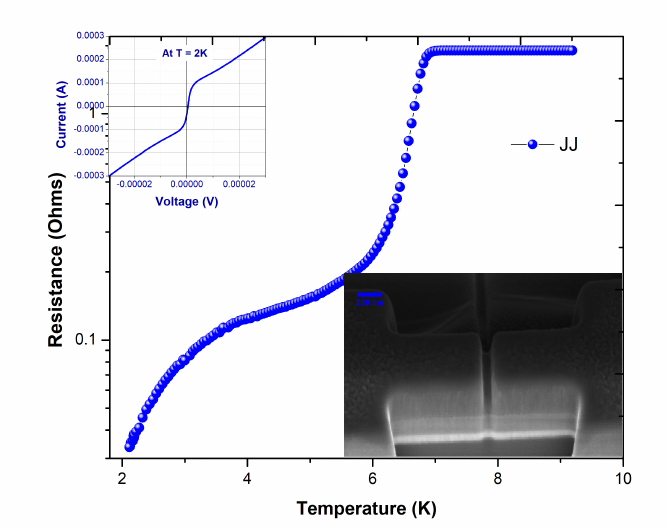
\includegraphics[width=10cm,bb = 0 0 200 100, draft, type=eps]{/run/media/ashwin/Data/Sandbox/Ash_docs/NISER/Thesis/Sem1-report/JJ.jpg}\caption{RT graph for a Cu(100nm)Nb(150nm) Josephson junction. The inset shows
an SEM image of the measured JJ \label{fig:RT-graph-for}}
\end{figure}
The first transition indicates the superconducting transition of the
Niobium layer, and the second transition explains the proximitisation
of the weak link. The resistance $R_{n}$ at 9K (above $T_{c}$) and
$R_{L}$at 2K are noted and the sample is cooled back to sub 2K. $R_{n}$is
the normal resistance and indicates that the device is out of the
superconducting regime. Once the devices cool down to 2K the current-voltage
characteristics of the device is measured by sweeping current from
-$I_{n}$ to +$I_{n}$, where $I_{n}$ is the current for which the
device yields the resistance $R_{n}$ at 2K, ie. the device switches
to the normal regime. The I-V curves have the typical JJ behavior
and is plotted in Fig \ref{fig:IV-graph-for}.
\begin{figure}[H]
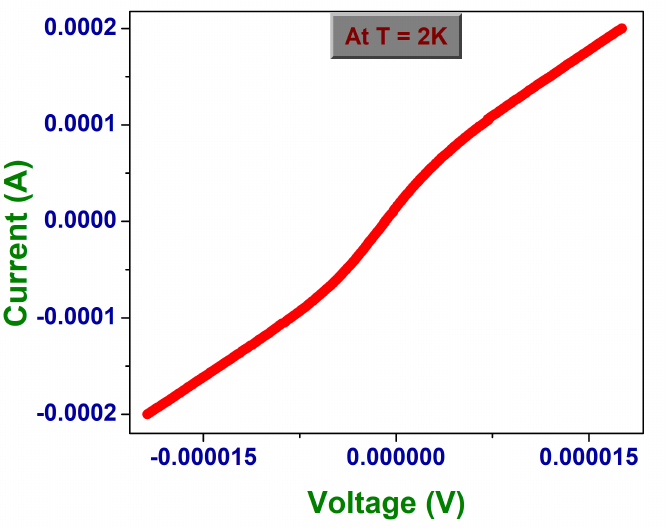
\includegraphics[width=10cm,bb = 0 0 200 100, draft, type=eps]{/run/media/ashwin/Data/Sandbox/Ash_docs/NISER/Thesis/Sem1-report/IV Pt20 CuNbJJ 2k.jpg}\caption{IV graph for a Cu(100nm)Nb(150nm) Josephson junction \label{fig:IV-graph-for}}
\end{figure}
 $I_{c}$ of the device and the electrodes were extracted using the
python scripts mentioned in section \ref{subsec:Automation-of-}.

In Fig \ref{fig:IV-graph-for} the IV curve of a Nb/Cu Josephson Junction
is shown. Once the device $I_{c}$ is found, the device is cooled
to 2K and then supplied with $I_{c}$ current, and the junction voltage
is measured while ramping the magnetic field from +250 Oe to -250
Oe ( positive cycle ) and then from -250Oe to 250Oe ( negative cycle
) at 2K. This gives us magnetoresistance as a function of the applied
magnetic field. The magnetoresistance as a function of applied magnetic
field is expected to have a diffraction pattern for JJ. This was explained
in the theoretical sections above.

\begin{figure}[H]
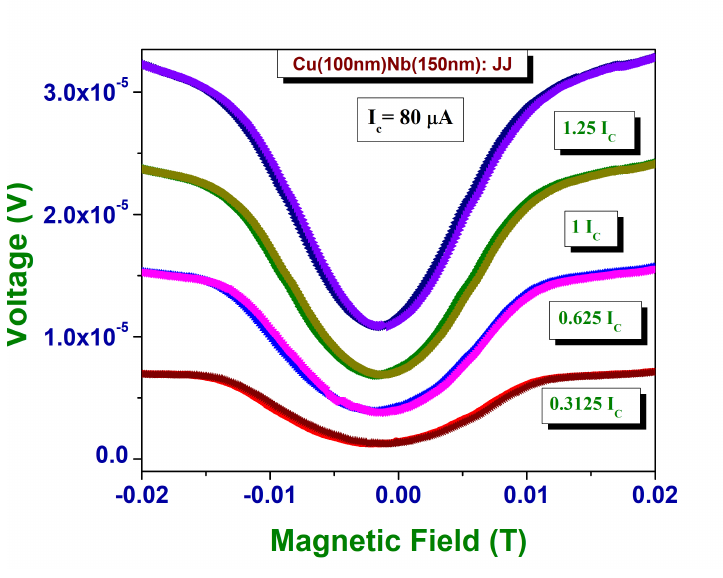
\includegraphics[width=10cm,bb = 0 0 200 100, draft, type=eps]{/run/media/ashwin/Data/Sandbox/Ash_docs/NISER/Thesis/Sem1-report/VH CuNbJJ 2k.jpg}\caption{Magnetoresistance of the patterned Nb/Cu Josephson junction device
in low magnetic fields for different values of junction currents\label{fig:Magnetoresistance-of-the-1}}
\end{figure}

\begin{figure}[H]
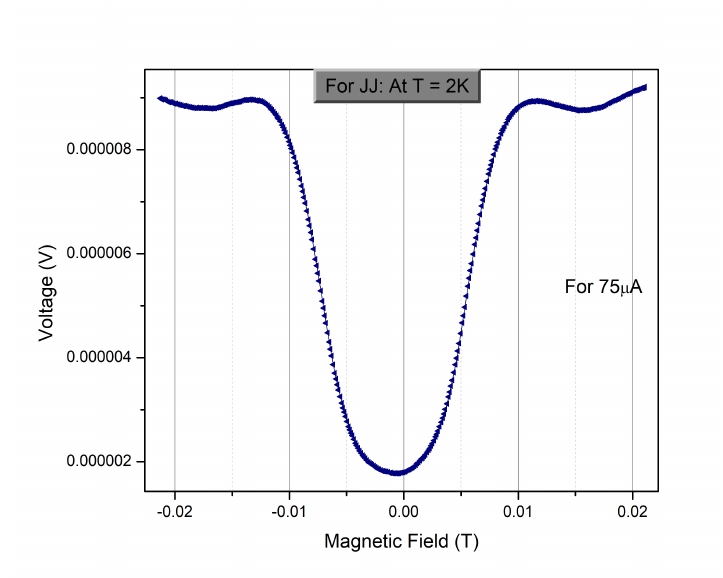
\includegraphics[width=10cm,bb = 0 0 200 100, draft, type=eps]{/run/media/ashwin/Data/Sandbox/Ash_docs/NISER/Thesis/Sem1-report/JJ VH.jpg}\caption{Magnetoresistance of the patterned Nb/Cu Josephson junction device
in low magnetic fields\label{fig:Magnetoresistance-of-the-1}}
\end{figure}

In Fig \ref{fig:Magnetoresistance-of-the-1} , we examine the magnetoresistance
of the patterned Nb/Cu Josephson junction device in low magnetic fields
(|H| < 300 Oe) and at its $I_{c}$. We find that the main lobe of
the positive and the negative cycle overlap completely and there is
no shift of the main lobe from origin as one would expect for a normal
S-N-S junction. Fig \ref{fig:Magnetoresistance-of-the-1} is a plot
of Junction voltage as a function of magnetic field for another patterned
Nb/Cu Josephson junction device in low magnetic fields for different
values of junction currents. One can observe that higher currents
increase the height of the lobes however the ratio of the first (main)
lobe to the second lobe remains constant. This pattern was also confirmed
with the simulation results.

\subsection{Comparing simulation with experimental data}

In Fig \ref{fig:Magnetoresistance-of-the-1}. Magnetoresistance of
the patterned Nb/Cu Josephson junction device (which exhibits first
harmonics only) in low magnetic fields for different values of junction
currents is plotted. This plot is similar to the $VH$ plot obtained
from the simulation for Q=1.5 with only first harmonics enabled (Fig
\ref{fig:Plots-of-VHs-1.5-1} (bottom) ). This further confirms the
equivalence between $VH$ plot obtained experimentally and $VH$ plot
obtained from simulations, Thus establishing that the $VH$ plot obtained
experimentally confirms the typical characteristic of the Josephson
junction. 

\section{Processing experimental data}

\subsection{Automation of $I_{c}$ extraction\label{subsec:Automation-of-}}

Once the IV simulation is done, in order to aggregate data for $I_{c}$as
a function of applied magnetic field $H$ ($I_{c}H)$ and Junction
voltage at as a function of applied magnetic field $H$ ($VH$), One
must first set the process for identifying $I_{c}$. In case of simulations,
since the data is quite smooth, we could choose a junction voltage
which corresponds to Ic for one run and find the current value for
that particular voltage on other runs. This is essentially a horizontal
slice of the IV curve in Fig \ref{fig:IV-Q}. For experimental data,
there is another way to define the $I_{c}$of a given PPMS data.

$I_{c}$ of the junction were extracted from this data by running
through a python script that takes in the I-V data, calculates dV/dI,
and applies a Savitzky--Golay filter of first-order to obtain $d^{2}I/d^{2}V$
and find the current ($I_{c}$) for which $d^{2}I/d^{2}V$ in both
the positive and negative side and averages them. For normal Josephson
junction the position of peak of $dI/dV$ is a good marker of the
$I_{c}$, however in cases where the junction resistance is high,
$dI/dV$ might not be clear enough to mitigate this peaks of $d^{2}I/d^{2}V$
is a better marker of $I_{c}$ A sample graph of $dI/dV$ and $d^{2}I/d^{2}V$
for a I vs V curve measured on a Josephson junction is shown in Fig
\ref{fig:findIc}.
\begin{figure}[H]
\centering{}\includegraphics[width=15cm]{samplePlot}\caption{A sample graph of $dI/dV$ and $d^{2}I/d^{2}V$ for a I vs V curve
measured on a Josephson junction. The $I_{c}$ extracted from the
graph is 140$\mu A$ \label{fig:findIc}}
\end{figure}
 The code for the python script is available \href{https://github.com/iamashwin99/JJ-Ic-finder}{here}
and a web app based on the same is hosted at \href{https://jj-ic-finder.herokuapp.com/}{jj-ic-finder.herokuapp.com}

The web app also provides quick access to multiple data visualizations
like area plot,bar plot,line plot, hist plot, scatter plot etc. A
screenshot of the web-app in use for visualizing the IV of an experimental
data of JJ is shown in Fig\ref{fig:iv-viz}.

\begin{figure}[H]
\centering{}\includegraphics[width=10cm]{web-app-sc}\caption{A screenshot of the web-app in use for visualizing the scatter plot
of Josephson junctions IV \label{fig:iv-viz}}
\end{figure}
 

\subsection{Inferring $I_{c}$ behavior via repetitive IV measurement}

The characteristic signature of a Josephson junction, apart from its
current voltage relation (IV) is the Critical current $I_{c}$dependence
on the applied magnetic field H ( $I_{C}$vs H or $I_{C}H$).

The PPMS in the lab has builtin recipes only for DC measurement and
as such DC measurements like IV are relatively slower (1 IV scan in
10-15 minutes on good resolution). Thus getting data for $I_{c}H$
would require multiple IVs to be measured at a sweep of magnetic field
H. This would take almost a day per device on a decent resolution
and thus cant be done frequently. The more easier measurement would
be to set and constant current (say the $Ic$ at zero magnetic field)
then measure the Voltage as a function of changing magnetic field
( V vs H or VH ) however, there is little literature regarding the
VH relation (or magneto resistance ) of a Josephson junction. In order
to verify the correlation between the $I_{C}H$ and $VH$ signatures
of a Josephson junction, apart from the simulation methods, multiple
IV seeps of a Josephson Junction were setup at varying magnetic field
were taken, and a python script mentioned in the previous sub section
was used to identify the $I_{C}$ for each $H$. The plots of these
$I_{C}H$ and $VH$ data is shown in Fig . The VH data for these junctions
have some parts which are offset due to random phase jumps. On comparison,
one can make out the Fraunhofer like pattern in both plots at the
same magnetic field points, the main lobe width and the secondary
lobe width are identical.

\begin{figure}[H]
\begin{centering}
\includegraphics[width=10cm]{IcH-JJ4}
\par\end{centering}
\centering{}\includegraphics[width=10cm]{VH-JJ4}\caption{Plots of $I_{C}H$ (analyzed from data) and $VH$(directly measured)
for a Niobium/Copper/Platinum Josephson junction (Sample no 4 from
run SP169)\protect \\
One can make out the Fraunhofer like pattern in both plots at the
same magnetic field points. \label{fig:jj4}}
\end{figure}
 

\begin{figure}[H]
\begin{centering}
\includegraphics[width=10cm]{IcH-JJ5}
\par\end{centering}
\centering{}\includegraphics[width=10cm]{VH-JJ5}\caption{Plots of $I_{C}H$ (analyzed from data) and $VH$(directly measured)
for a Niobium/Copper/Platinum Josephson junction (Sample no 5 from
run SP169)\protect \\
One can make out the Fraunhofer like pattern in both plots at the
same magnetic field points. \label{fig:jj4-1}}
\end{figure}
 

Apart from this measurement, an attempt was made to setup Keithley
6221 - AC current source and Keithley 2182a - Nanovoltmeter in differential
conductance mode.

This method involves sweeping a linear staircase profile with an alternating
current. The differential current, dI, is the amplitude of the alternating
portion of the current as shown in Fig \ref{fig:dcon}. Throughout
the test, the differential current remains constant. A Trigger Link
cable synchronises the current source with the nanovoltmeter. The
nanovoltmeter calculates the delta voltage between consecutive steps
after measuring the voltage at each current step. To determine the
differential voltage, dV, each delta voltage is averaged with the
previous delta voltage. dI/dV may now be used to calculate the differential
conductance, dG. \cite{kiethley-dcon}

\begin{figure}[H]
\centering{}\includegraphics[width=10cm]{dcon-6221}\caption{A plot of the applied current bias in the differential conductance
setup\label{fig:dcon}\cite{kiethley-dcon}}
\end{figure}
 

The Labview program provided by the instrument manufacturer required
the connection to the 6221 via a GPIB interface, however the 6221
was connected to a system with no GPIB port. In order to over come
this, communication was setup serially via the Ethernet ports and
python serial communication library. A graphical user interface (GUI)
was built built to control the communication and perform the differential
conductance as shown in Fig \ref{fig:A-GUI-setup}.

\begin{figure}[H]
\centering{}\includegraphics[width=13cm]{dcon-gui}\caption{A GUI setup to control the differential conductance setup\label{fig:A-GUI-setup}}
\end{figure}
 

The data provided by the instrument is differential conductance, dG
as a function of applied current. The experiment needed dG as a function
of junction voltage and the data acquired by the device was quite
unreliable and noisy, thus this method was not used further. A better
way to do differential conductance would be to use a lock-in amplifier.

\section{Conclusion}

The main goal of the thesis was to establish equivalence between the
$I_{c}H$and $VH$ (magnetoresistance) characteristics of a Josephson
junction ( with and without the second harmonics), then further establish
the experimental $VH$ plot and the simulated $VH$ plot.

For the first part, the simulation was setup by solving the ODE with
input similar to the experimental input of, sweeping the current while
equilibrating the system at each step and then repeating this over
multiple magnetic field, then further analysing this data to obtain
$I_{c}H$and $VH$ plots. For the second part, experimental data was
gathered similar to the simulation steps (calculating IV data for
multiple magnetic field ) and then analysed to to obtain $I_{c}H$and
$VH$ plots, the results obtained from this was matched with the simulation
results.

In both of the above method, the equivalence between the $I_{c}H$and
$VH$ (magnetoresistance) characteristics of a Josephson junction
was confirmed and was also matched with the experimental results.
One could carry out the study further by:
\begin{itemize}
\item Carrying out a simulation analysis with respect to $\beta_{c}$and
compare it with the results obtained through Q
\item Simulation of other exotic CPR such as sin($\phi/2$)
\item The simulation currently takes about 2hrs for sweeping magnetic fields
linearly spaced between $-2\frac{\phi}{\phi_{0}}$ and $2\frac{\phi}{\phi_{0}}$
. An improvement in the simulation/integration time by using numba
decorators for numpy-python modules could be made, for instance Scipy's
odeint integration will be slow if the right-hand side of an ODE integration
is slow. The numba package, which translates python code into machine
code using LLVM - which means it's very fast, it can speed up the
right-hand side. Even a very simple ODE can be sped up by several
factors.
\item A study could be done on finding the Q value of the experimental junction,
by fitting the IV with Q as a parameter
\item The differential conductance measurement could be setup using a lockin
amplifier.
\end{itemize}
\newpage{}

\bibliographystyle{ieeetr}
\addcontentsline{toc}{section}{\refname}\nocite{*}
\bibliography{report}

\end{document}
